%!TEX root = ../TTK4900-MHT.tex
\chapter{Results}\label{chapter:results}
The performance evaluation of any tracking system is difficult since the degrees of freedom are very large and there are no single obvious performance metric~\cite{Schuhmacher2008}. There are however two distinct testing methods found in the literature, pure Monte Carlo testing and situation/scenario testing. The first being that parameters like number of tracks, start position, velocity, manoeuvring, missed detections and clutter all are randomly selected and repeated many times. This approach is reasonable from a stochastic point of view, but it does not necessary create realistic tracking scenarios for in our case a maritime environment. The second approach is to create one or more scenarios which then is simulated with random variables like missed detections and clutter measurements. This approach is vulnerable to the created scenarios, since the design can heavily impact the measured performance. However, this method allows for construction of very specific situations where it is desirable to test multiple tracking system on the same custom created situation for comparison purposes.

The second approach is used in this work based on its ability to run user defined scenarios and its perceived more realistic behaviour. 

\section{Testing scheme}
The performance evaluation of any MHT system is tedious in that it is necessary to test very many different situations to get a good understanding of how the system performs in a broad sense. The two largest factors contributing to the difficulty is the random nature of the clutter and lost detections. It is also desirable to evaluate the initialization and tracking performance under both varying environmental (external) conditions and tuning (internal) setting. We want good tracking of targets with low probability of detection in cluttered environment, and have a runtime no larger than the radar rotation period. The initialization module must be able to detect targets with probability of detection lower than unity without initializing too many false tracks into the MHT algorithm. The testing following is separated into two parts; initialization and tracking.

\section{Scenario}\label{sec:scenario}
All simulations in this work is based on a generated scenario, shown in Figure~\ref{fig:test_scenario}, with black dots marking the initial time and position of the targets. The radar range is 5500 meter (\textasciitilde 3 \glspl{nm_acr}), which gives an area of surveillance of approximately 95 square km. The scenario contains 16 targets, which all starts inside the observable area of the radar. The scenario contains a mixture of fast and slow moving vessels, some with sharp turns and some almost at stand still. Table~\ref{tab:init_states} show the initial states of all targets, and the true path is generated once from these initial values.
\begin{figure}
\centering
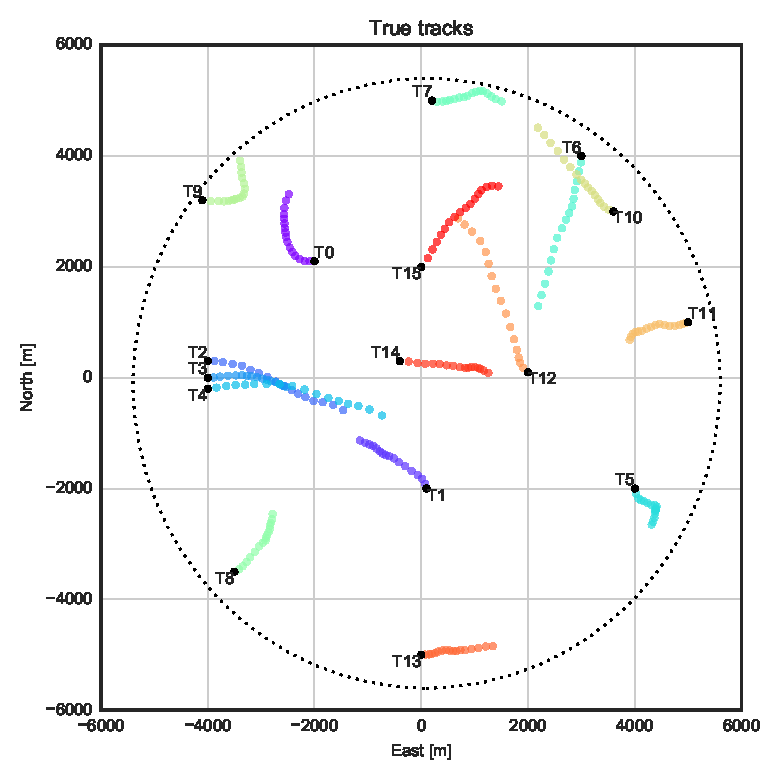
\includegraphics{Figures/plots/ScenarioTruth.pdf}
\caption{True tracks}\label{fig:test_scenario}
\end{figure}
\begin{table}
\centering{}
\begin{tabular}{c c c c c}
\bfseries Target & \bfseries North & \bfseries East & \bfseries North speed & \bfseries East speed \\ 
\toprule
\csvreader[head to column names,respect percent=true]{{Figures/plots/Scenario_Initial_State.csv}}{}
{\T{} & \NP{} & \EP{} & \NS{} & \ES{} \\}
\end{tabular}
\caption{Initial states}\label{tab:init_states}
\end{table}

From this base scenario, five scenarios where generated with different AIS configuration on the vessels, see Table~\ref{tab:ais_scenarios}. The first scenario represents the baseline with only radar information available, whereas the rest have some level of AIS information. Scenario 1 adds 50\% class B AIS transmitters, and is representing a situation where all the targets are smaller vessels with some voluntarily installed AIS transceivers. In scenario 3, all vessels have AIS class B installed. This scenario represents a best case situation regarding yacht and leisure vessels from an autonomous anti collision perspective and is only realistic if AIS class B were to be mandatory for these vessel classes. Scenario 2 is the same as scenario 1, with the difference that the vessels have class A transmitters in stead of class B. This gives them higher and smarter rate of transmission (see \Cref{tab:classA_reporting_intervals,tab:classB_reporting_intervals}), which in theory should improve tracking. This scenario can be viewed as a few commercial vessels travelling in between a large group of yachts. The last scenario, where all targets are equipped with class A transmitters is the ultimate situation for any fusion tracking system. This case would be realistic in a crowded professional working area, for instance harbours, fishing areas and off-shore installations.

\Cref{fig:measurements_overlaid} show all radar measurements for an entire scenario for the different clutter level overlaid. 
\begin{table}
\centering
\csvautotabular{{Figures/plots/Scenario_AIS_State.csv}}
\caption{AIS class scenario configuration}\label{tab:ais_scenarios}
\end{table}

\begin{figure}
 \centering
 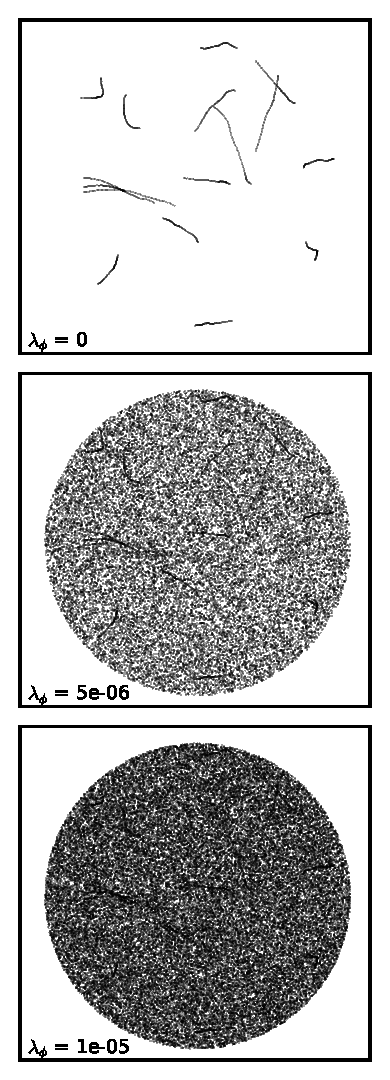
\includegraphics{Figures/plots/ScenarioOverlaid}
 \caption{Scenario measurements overlaid}\label{fig:measurements_overlaid}
\end{figure}

\section{Simulation}
Both initialization- and tracking performance are averaged over a set of 25 Monte Carlo simulations with differently seeded clutter- and missed radar detections. All simulations were done with a sampling interval at 2.5 seconds (24 \gls{rpm}), which is a common rotation speed on a coastal maritime radar. Each of the 540 initialization variations and 180 track performance simulations where run on a dual Intel i7--6700 server running Linux Ubuntu with \gls{ssd} storage and 64 GB \gls{ram}.

\section{Initialization results}
The first performance metric for the initialization module is how long time it takes to initialize the correct tracks, which is tested under a range of internal and external conditions, see (\ref{eq:init_test_table}). All 108 combinations of these parameters were simulated on all five scenarios (Table~\ref{tab:ais_scenarios}), which are the same routes but with different \gls{ais} configurations. Each of these 540 variations were repeated 30 times, and from these 16,200 simulations, the average time to initiate true targets and amount of erroneous targets are calculated.
\begin{equation}\label{eq:init_test_table}
\begin{split}
\V{P_D} &= \begin{bmatrix} 0.9 & 0.8 & 0.6 \end{bmatrix} \\
(m/n) &= \begin{bmatrix} 	(1/1) & (1/2) & (1/3) & (1/4) \\
							(2/2) & (2/3) & (2/4) & (2/5) \\
							(3/3) & (3/4) & (3/5) & (3/6)
		   \end{bmatrix} \\
\V{\lambda_\phi} &= \begin{bmatrix} 0 & 5\cdot10^{-6} & 1\cdot10^{-5}\end{bmatrix}
\end{split}
\end{equation}

A track is categorized as correctly initialized if the position difference between the true track and the initial track (\ref{eq:euclidian_distance_vector}) is less than a threshold. All initial tracks that do not correspond to true tracks, are categorized as erroneous. To analyse the impact of the erroneous tracks, the lifespan of falsely initiated tracks are investigated to see whether they die out at the same rate as they are initiated, or if they accumulate.

\Cref{fig:init0_time_2-5,fig:init0_time_2-4,fig:init0_time_2-3,fig:init0_time_2-2,fig:init0_time_1-2,fig:init0_time_1-4,fig:init0_time_1-1,fig:init0_time_3-4,fig:init0_time_1-3,fig:init0_time_3-3,fig:init0_time_3-6,fig:init0_time_3-5}, \cref{fig:init1_time_2-5,fig:init1_time_2-4,fig:init1_time_2-3,fig:init1_time_2-2,fig:init1_time_1-2,fig:init1_time_1-4,fig:init1_time_1-1,fig:init1_time_3-4,fig:init1_time_1-3,fig:init1_time_3-3,fig:init1_time_3-6,fig:init1_time_3-5}, \cref{fig:init2_time_2-5,fig:init2_time_2-4,fig:init2_time_2-3,fig:init2_time_2-2,fig:init2_time_1-2,fig:init2_time_1-4,fig:init2_time_1-1,fig:init2_time_3-4,fig:init2_time_1-3,fig:init2_time_3-3,fig:init2_time_3-6,fig:init2_time_3-5}, \cref{fig:init3_time_2-5,fig:init3_time_2-4,fig:init3_time_2-3,fig:init3_time_2-2,fig:init3_time_1-2,fig:init3_time_1-4,fig:init3_time_1-1,fig:init3_time_3-4,fig:init3_time_1-3,fig:init3_time_3-3,fig:init3_time_3-6,fig:init3_time_3-5} and \cref{fig:init4_time_2-5,fig:init4_time_2-4,fig:init4_time_2-3,fig:init4_time_2-2,fig:init4_time_1-2,fig:init4_time_1-4,fig:init4_time_1-1,fig:init4_time_3-4,fig:init4_time_1-3,fig:init4_time_3-3,fig:init4_time_3-6,fig:init4_time_3-5} show the initialization performance for Scenario 0 to 4 respectively, averaged over the Monte Carlo simulations. Their first plot is the share of true track correctly initialized over time, whereas the second and third plot is the amount and density of falsely initiated tracks. The share of correctly initialized tracks is defined as the number of true tracks that have been initialized minimum one time divided on the total number of true tracks. This prevents re-initialized true tracks to be counted more than one time, and an initialization share on 100\% means that all tracks have been initialized correctly at least one time. The difference between the two last plots is that the first is an accumulation of false track over time, while the last is the number of erroneous tracks alive at that time. These data are summarized in \Cref{fig:init_performance_scenario0,fig:init_performance_scenario1,fig:init_performance_scenario2,fig:init_performance_scenario3,fig:init_performance_scenario4} to better evaluate their performance over the set of variations. 

For each scenario and initialization setting (m/n), an average cost of the variations (\gls{Pd} and \(\lambda_\phi \)) were calculated based on (\ref{eq:init_score_function}). \(t_{80\%}\) is the time it took to reach 80\% correctly initialized true tracks, and variations that never reaches 80\% is penalized with a high `initialization time' selected to match the worst scenarios. A lower cost means that the time it took to correctly initialize 80\% of the true tracks and the average number of false tracks alive where both low. An increase in either time or number of false tracks would increase the cost. To better see the nuances close to zero, the plot show the normalized square root of the cost, were the normalization constant is the highest cost among all the scenario's tuning parameters. The normalization is done to keep in numeric values in a defined set since the cost function is only a representation of the performance between the different tuning setting. 
\begin{equation}\label{eq:init_score_function}
Cost = t_{80\%} (1 + n_{False Track})
\end{equation}

From \Cref{fig:init_performance_scenario0,fig:init_performance_scenario1,fig:init_performance_scenario2,fig:init_performance_scenario3,fig:init_performance_scenario4} we see that each M row has a peak (low cost) and edges with higher costs. (2/3) and (2/4) are overall good values with a balance between initialization time and the amount of erroneous tracks. We can also see that the AIS aided initializations are all performing better than the pure radar scenario. 
\begin{figure}
 \centering
 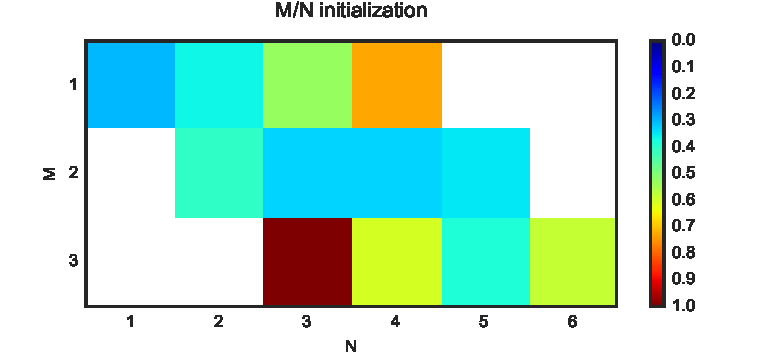
\includegraphics{Figures/plots/Scenario0_Init-Performance.pdf}
 \caption{Scenario 0 --- Initiator performance}\label{fig:init_performance_scenario0}
\end{figure}

\begin{figure}
 \centering
 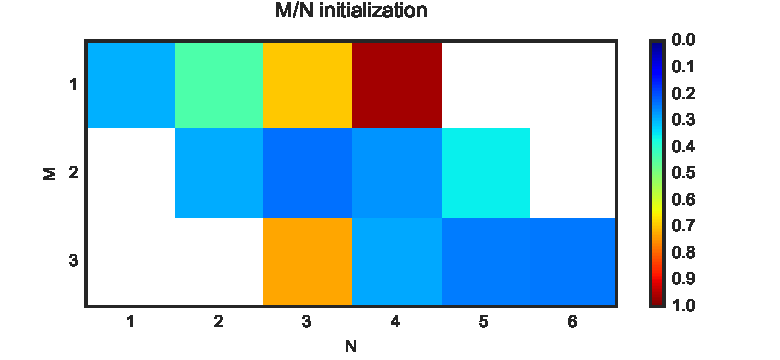
\includegraphics{Figures/plots/Scenario1_Init-Performance.pdf}
 \caption{Scenario 1 --- Initiator performance}\label{fig:init_performance_scenario1}
\end{figure}

\begin{figure}
 \centering
 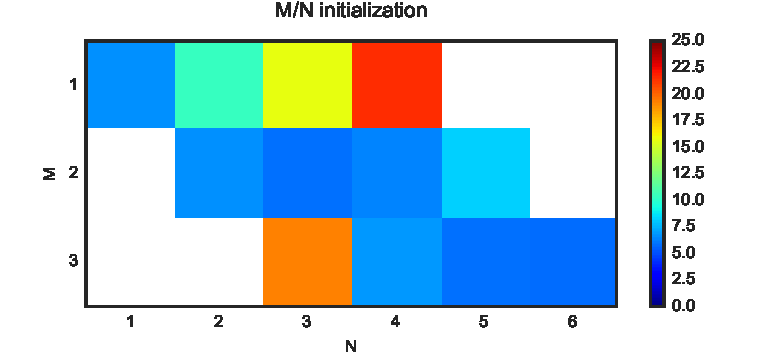
\includegraphics{Figures/plots/Scenario2_Init-Performance.pdf}
 \caption{Scenario 2 --- Initiator performance}\label{fig:init_performance_scenario2}
\end{figure}

\begin{figure}
 \centering
 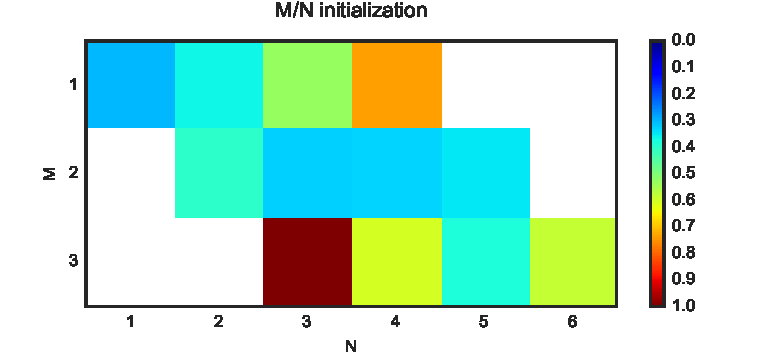
\includegraphics{Figures/plots/Scenario3_Init-Performance.pdf}
 \caption{Scenario 3 --- Initiator performance}\label{fig:init_performance_scenario3}
\end{figure}

\begin{figure}
 \centering
 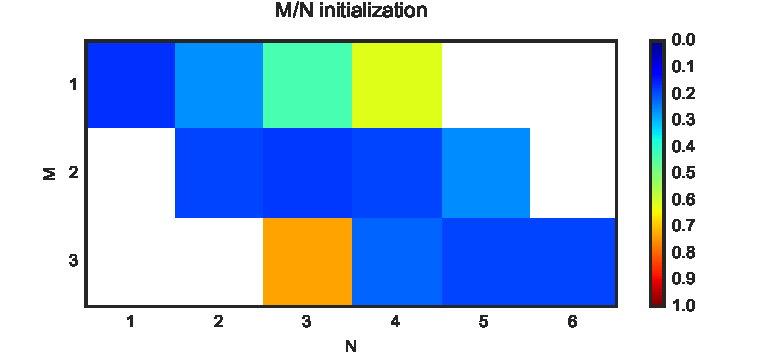
\includegraphics{Figures/plots/Scenario4_Init-Performance.pdf}
 \caption{Scenario 4 --- Initiator performance}\label{fig:init_performance_scenario4}
\end{figure}
\clearpage{}

\section{Tracking results}
When testing the tracking performance, it is desirable to remove the variable of initialization to better see difference in \emph{tracking} rather than \emph{initialization}. All simulations testing tracking performance are carried out with all targets correctly initialized at initial time, and with the initiator set to \( (2/4) \). The unused measurements from the tracking algorithm is processed by the initialization algorithm, giving lost targets a chance to get re-initialized, which is an important property for any safety critical system. For scenarios where \gls{ais} measurements are available, the unused \gls{ais} measurements are used to aid the initiator. Similar to the initialization testing, each of the five scenarios are tested under varying internal and external conditions (\ref{eq:tracking_test_table}). The 180 variations are repeated 30 times, giving rise to 5400 simulations from which the performance metrics are calculated. 
\begin{equation}\label{eq:tracking_test_table}
\begin{split}
\V{P_D} &= \begin{bmatrix} 0.9 & 0.8 & 0.6 \end{bmatrix} \\
\V{N} &= \begin{bmatrix} 1 & 3 & 6 & 9 \end{bmatrix} \\
\V{\lambda_\phi} &= \begin{bmatrix} 0 & 5\cdot10^{-6} & 1\cdot10^{-5} \end{bmatrix}
\end{split}
\end{equation}

Since the targets are initialized perfectly in every situation, we are interested in how good our system is able to \emph{maintain} the tracks. We measure this by means of the Euclidean distance between the estimated and true track (\ref{eq:euclidian_distance_vector}). The first track performance metric is the track loss percentage, where a track is considered correct as long as \(\Delta P \leq \varepsilon_p\) for a given threshold. If a track is deviating more than the threshold and never returns within the threshold again, it is considered lost at the time-step when it exceeded the threshold. If the track should converge after exceeding the threshold, it is considered restored at the time-step it is returning within the limit. Tracks that deviates more than \(10\varepsilon_p\) are considered lost at the time they exceeded \(\varepsilon_p\). This two step threshold is to allow tracks to dead reckon for a while without being registered as lost, while still dismiss tracks that are deviating away from the true track.
\begin{equation}
	\Delta P = \| \V{p}_{track}-\V{p}_{target} \|_2
\label{eq:euclidian_distance_vector}
\end{equation}

The second and closely related metric is the tracking percentage, where the total time a target is correctly tracked is summed up and compared with the existence time of the target. This situation is illustrated in Figure~\ref{fig:track_percentage} where a track is lost at (-2500,2600), and re-initialized at (-2500,2650). The track is considered lost at (-2500,2600), while the tracking percentage is also accounting the last track from (-2500,2650). This metric gives a more realistic measure of how likely targets are to be tracked, since lost tracks are assumed to often be re-initialized. 
\begin{figure}[H]
\centering
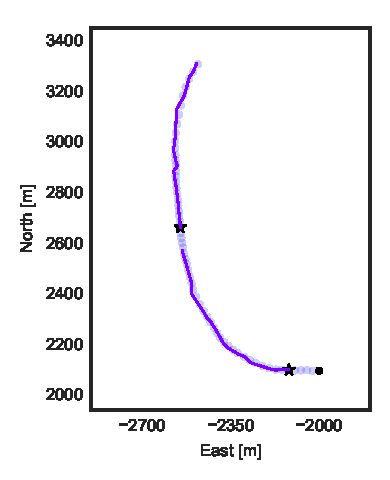
\includegraphics{Figures/plots/TrackingPercentageExample.pdf}
\caption{Tracking percentage, the sum of the total tracking time relative the existence time of the target}\label{fig:track_percentage}
\end{figure}

The third metric is how close the estimated track is to the true track on average. This is measured as the \gls{rmsd} of the entire track (\ref{eq:rmsd}), where \(n\) is the length of the track.
\begin{equation}\label{eq:rmsd}
RMSD = \sqrt{\frac{1}{n}\sum_{t=1}^{n}{(\Delta P_t)}^2}
\end{equation}



\subsection{Track loss}
From \cref{fig:scenario0_track_loss,fig:scenario1_track_loss,fig:scenario2_track_loss,fig:scenario3_track_loss,fig:scenario4_track_loss} we can see that the amount of lost tracks are very dependent on the probability of detection \gls{Pd} and window size (N). An interesting observation is the declination of lost tracks with increased clutter when N=1, which is most likely caused by clutter being gated and selected, giving the track a high enough score to not be terminated while still being similar enough to not loose the true track.

\Cref{tab:track_loss_improvement} show the improvement in track loss of the different AIS scenarios compared to the pure radar scenario, all for \(\lambda_\phi = 1\cdot 10^{-5}\). From this we can see that that the class of \gls{ais} has a large effect on the improvement when comparing the gain of all targets being equipped with class A versus class B \gls{ais}. It can also be seen that a minimum window size is necessary to achieve a substantial gain, this is probably because the tracking percentage is increasing but because of the low \gls{Pd} and the varying nature of \gls{ais} report interval most of the targets will still be lost at least one time.

\begin{table}[H]
\centering
\csvautotabular{{Figures/plots/Track_Loss_Improvement.csv}}
\caption{Track loss improvement relative pure radar}\label{tab:track_loss_improvement}
\end{table}

\begin{figure}
\centering
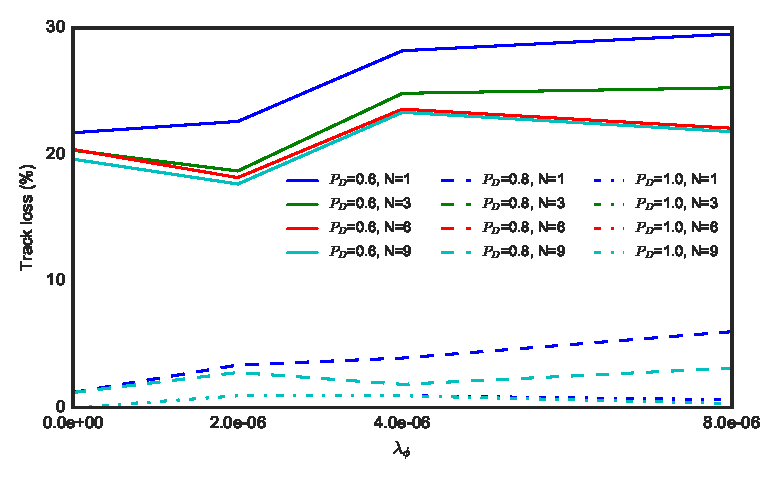
\includegraphics{Figures/plots/Scenario0_Tracking-TrackLoss.pdf}
\caption{Scenario 0 --- Track loss}\label{fig:scenario0_track_loss}
\end{figure}

\begin{figure}
\centering
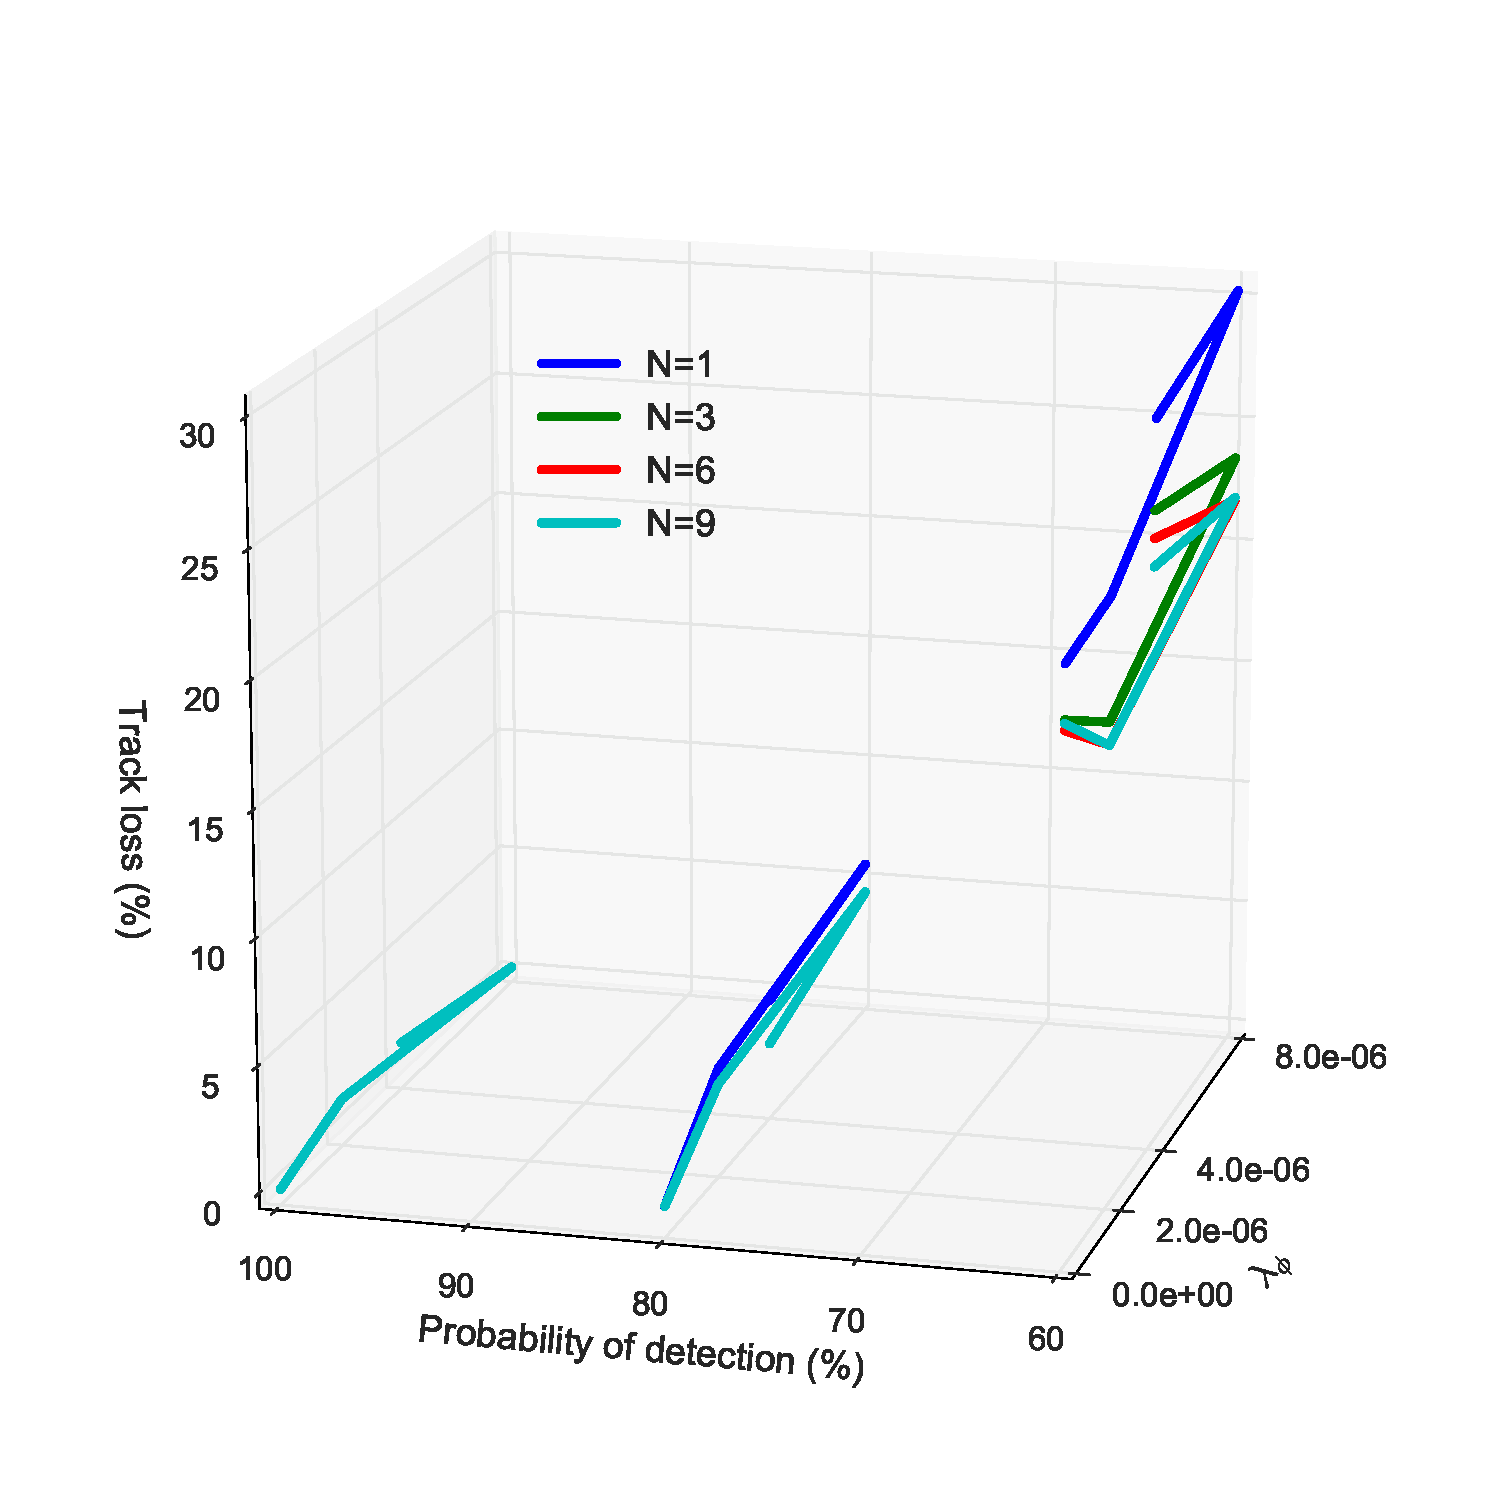
\includegraphics{Figures/plots/Scenario1_Tracking-TrackLoss.pdf}
\caption{Scenario 1 --- Track loss}\label{fig:scenario1_track_loss}
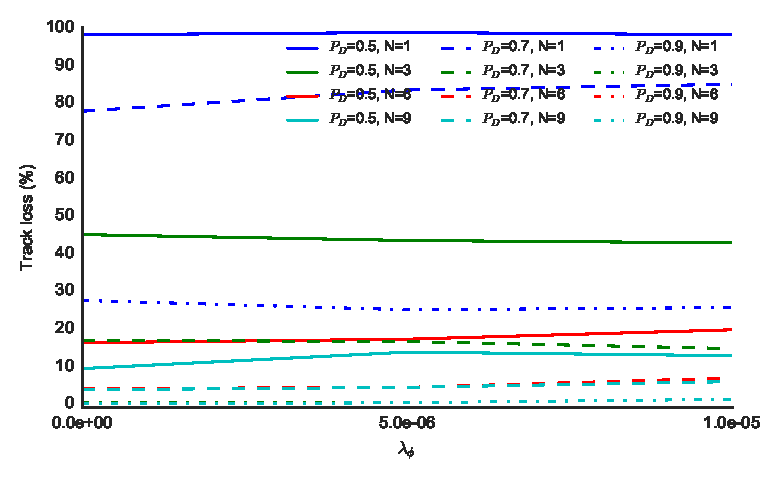
\includegraphics{Figures/plots/Scenario2_Tracking-TrackLoss.pdf}
\caption{Scenario 2 --- Track loss}\label{fig:scenario2_track_loss}
\end{figure}

\begin{figure}
\centering
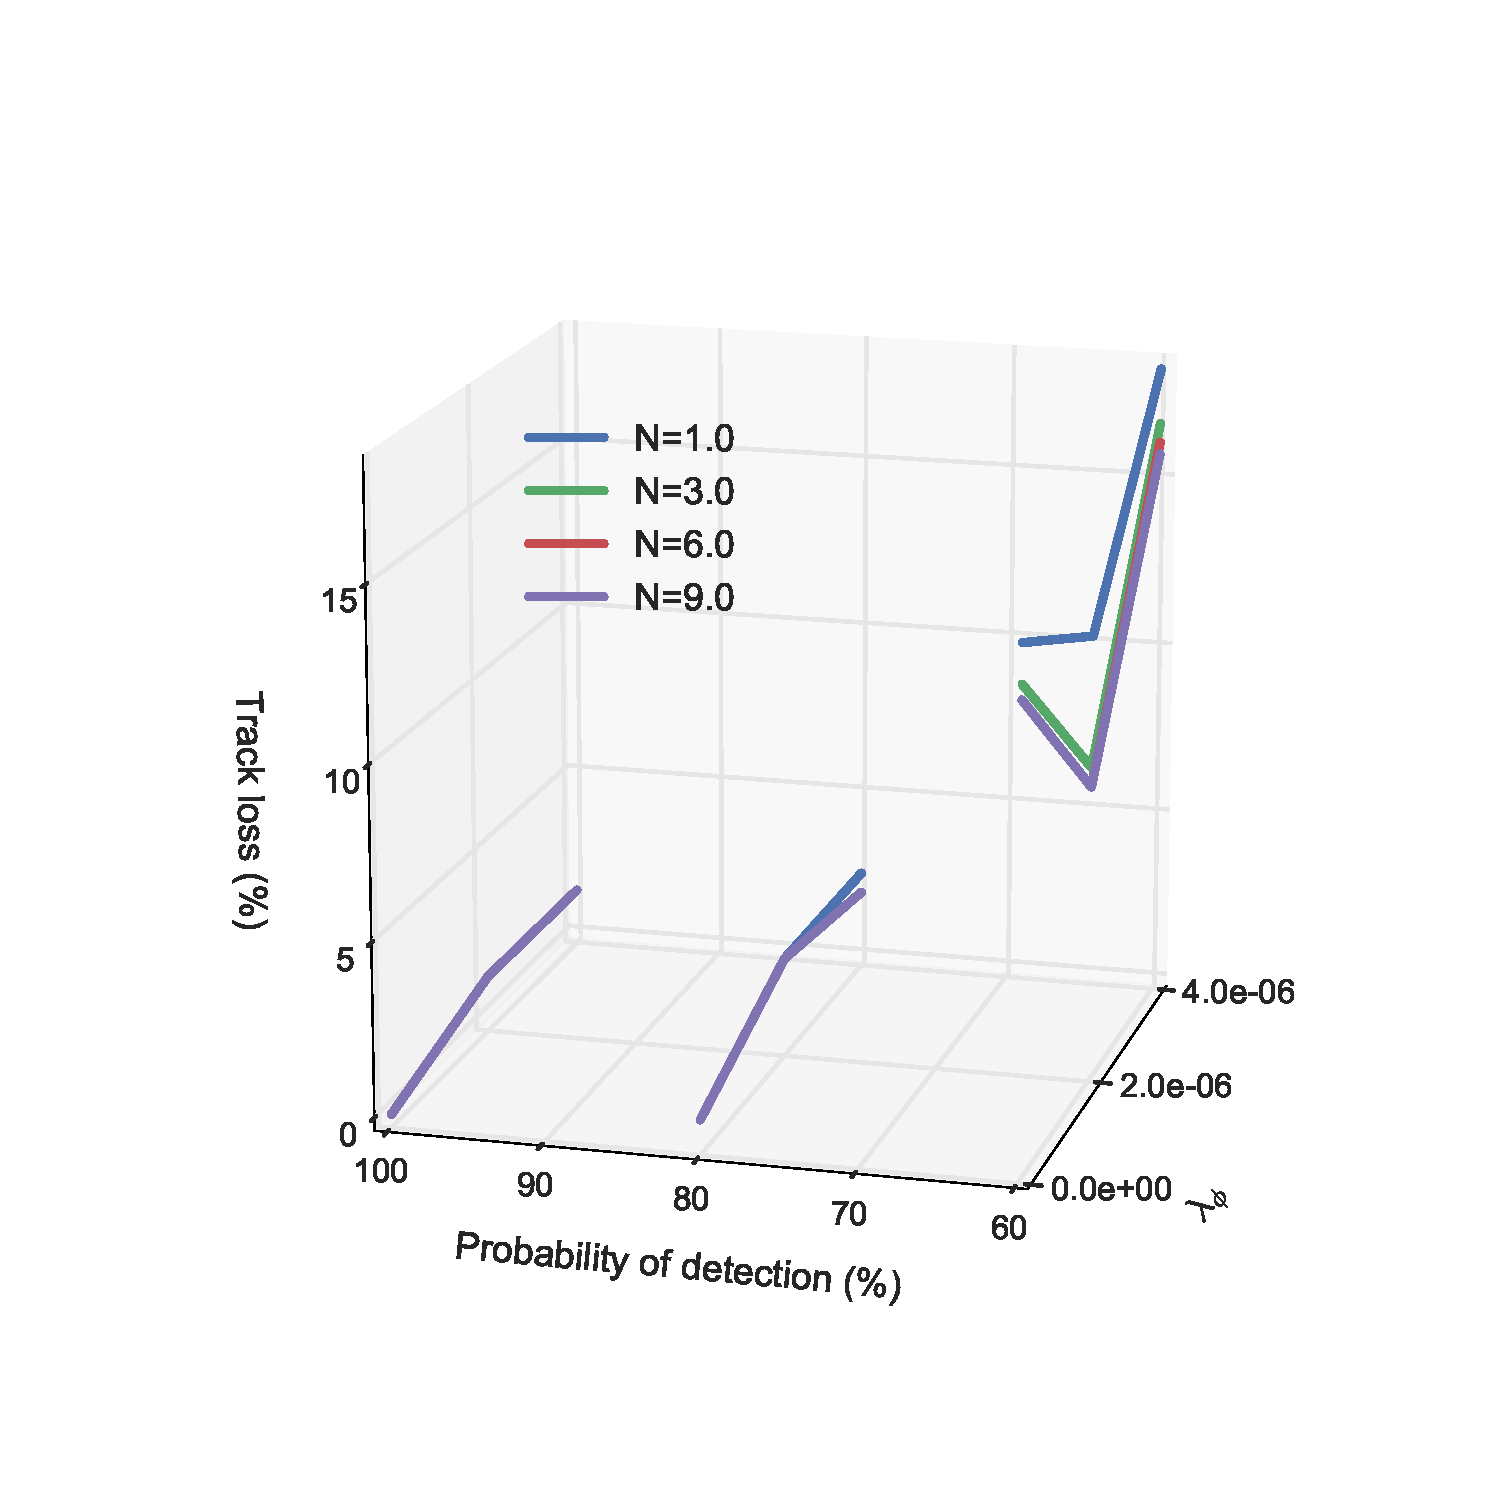
\includegraphics{Figures/plots/Scenario3_Tracking-TrackLoss.pdf}
\caption{Scenario 3 --- Track loss}\label{fig:scenario3_track_loss}
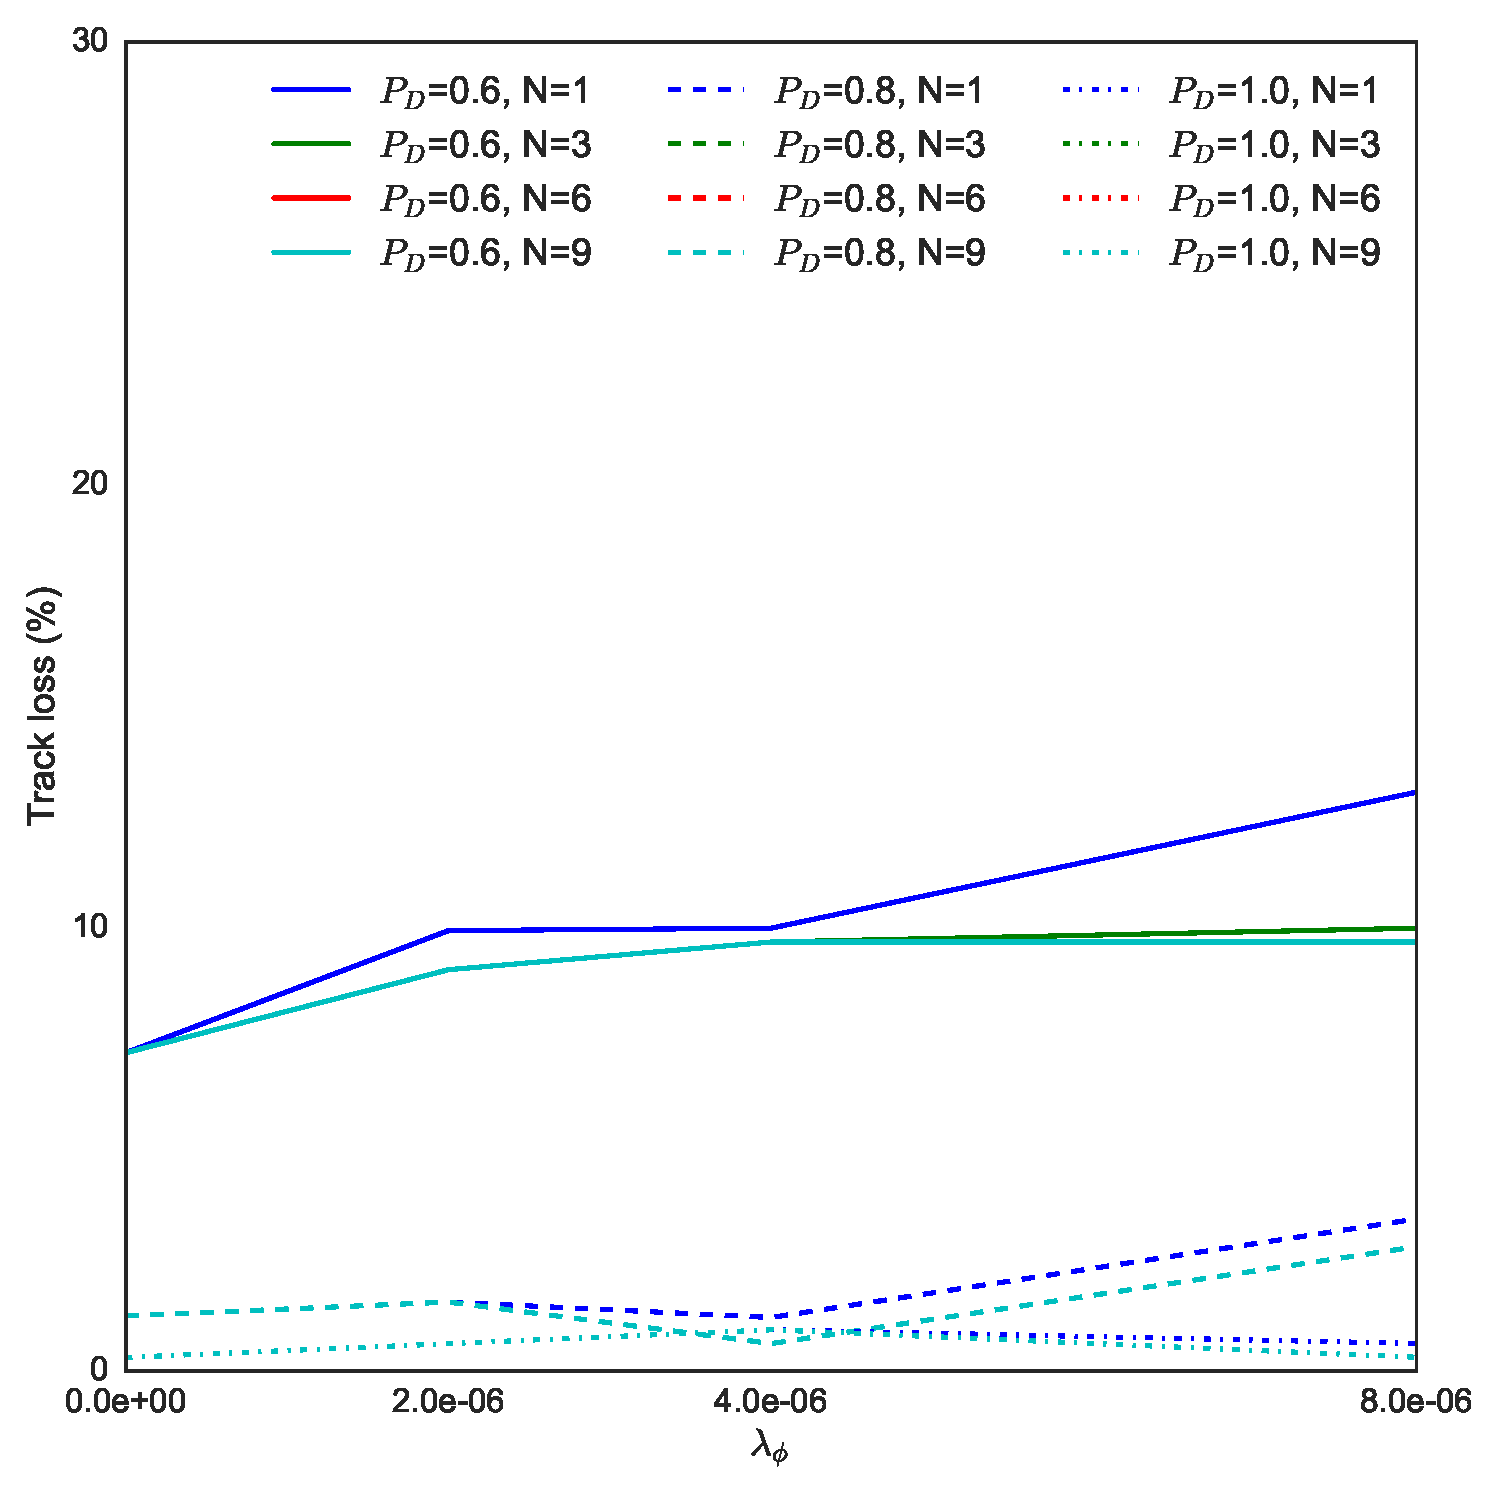
\includegraphics{Figures/plots/Scenario4_Tracking-TrackLoss.pdf}
\caption{Scenario 4 --- Track loss}\label{fig:scenario4_track_loss}
\end{figure}
\clearpage

\subsection{Tracking percentage}
\Cref{fig:scenario0_tracking_percentage,fig:scenario1_tracking_percentage,fig:scenario2_tracking_percentage,fig:scenario3_tracking_percentage,fig:scenario4_tracking_percentage} show the tracking percentage for scenario 0 --- 4. From these we can see a substantial increase in the tracking percentage for low \gls{Pd} and small window size when comparing the pure radar tracking with the \gls{ais} aided tracking. 
%The difference is biggest for N=1 in all cases, but since this is an very small window size will we focus our analysis on N=3 and 6 since these seems to be the sweet spot between runtime (\Cref{fig:scenario0_tracking_runtime,fig:scenario1_tracking_runtime,fig:scenario2_tracking_runtime,fig:scenario3_tracking_runtime,fig:scenario4_tracking_runtime}) and performance. 

\Cref{tab:tracking_percentage_improvement} list the improvements for the AIS scenarios compared to the pure radar baseline, all for \(\lambda_\phi = 1\cdot 10^{-5}\). From this we can see that the class of AIS equipment impacts the tracking performance more than the amount of AIS transmitters. It also shows that the benefits of AIS decreases with an increased \gls{Pd} and N. The performance gain for 70\% \gls{Pd} and higher is marginal for all cases except N=1 with class A \gls{ais}.
\begin{table}[H]
\centering
\csvautotabular{{Figures/plots/Tracking_Percentage_Improvement.csv}}
\caption{Tracking percentage improvement relative pure radar}\label{tab:tracking_percentage_improvement}
\end{table}

\begin{figure}
\centering
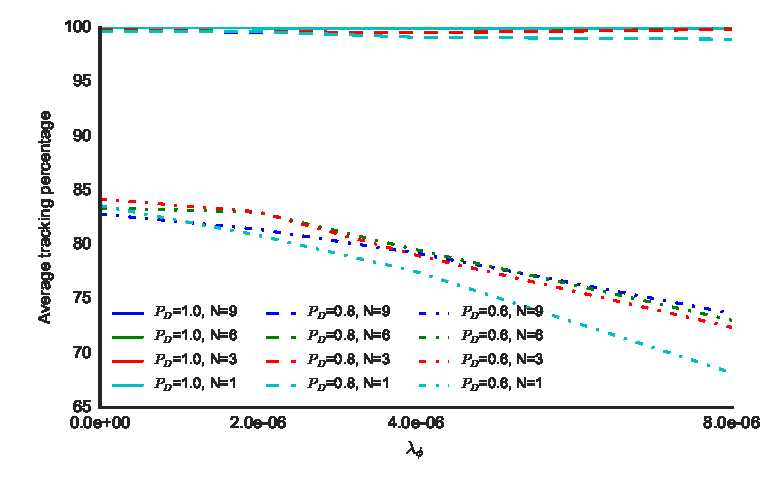
\includegraphics{Figures/plots/Scenario0_Tracking-TrackingPercentage.pdf}
\caption{Scenario 0 --- Tracking percentage}\label{fig:scenario0_tracking_percentage}
\end{figure}
\begin{figure}
\centering
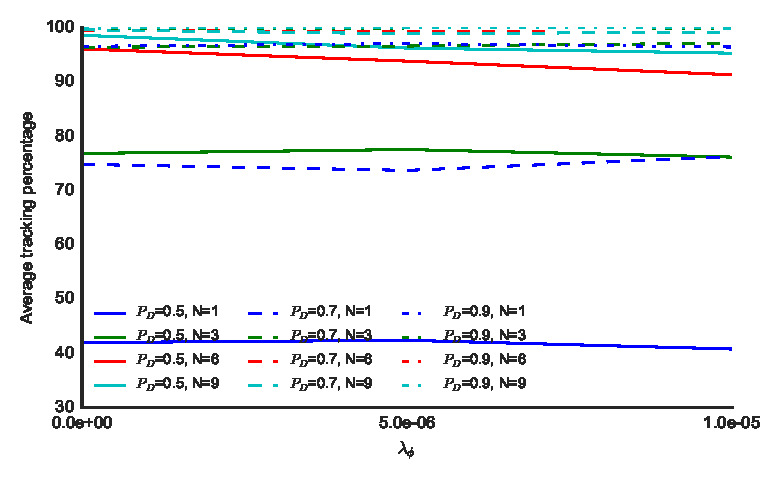
\includegraphics{Figures/plots/Scenario1_Tracking-TrackingPercentage.pdf}
\caption{Scenario 1 --- Tracking percentage}\label{fig:scenario1_tracking_percentage}
\end{figure}
\begin{figure}
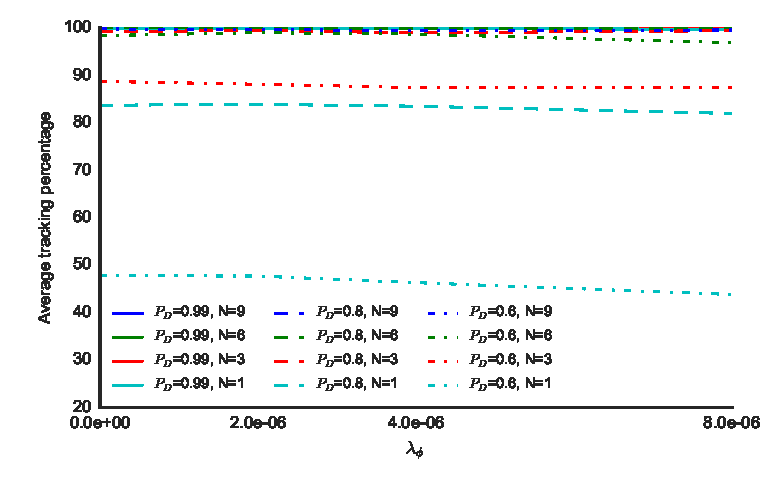
\includegraphics{Figures/plots/Scenario2_Tracking-TrackingPercentage.pdf}
\caption{Scenario 2 --- Tracking percentage}\label{fig:scenario2_tracking_percentage}
\end{figure}
\begin{figure}
\centering
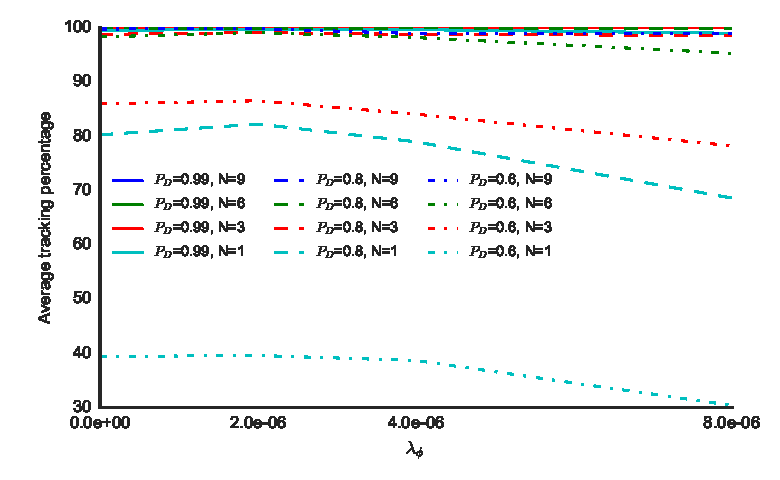
\includegraphics{Figures/plots/Scenario3_Tracking-TrackingPercentage.pdf}
\caption{Scenario 3 --- Tracking percentage}\label{fig:scenario3_tracking_percentage}
\end{figure}
\begin{figure}
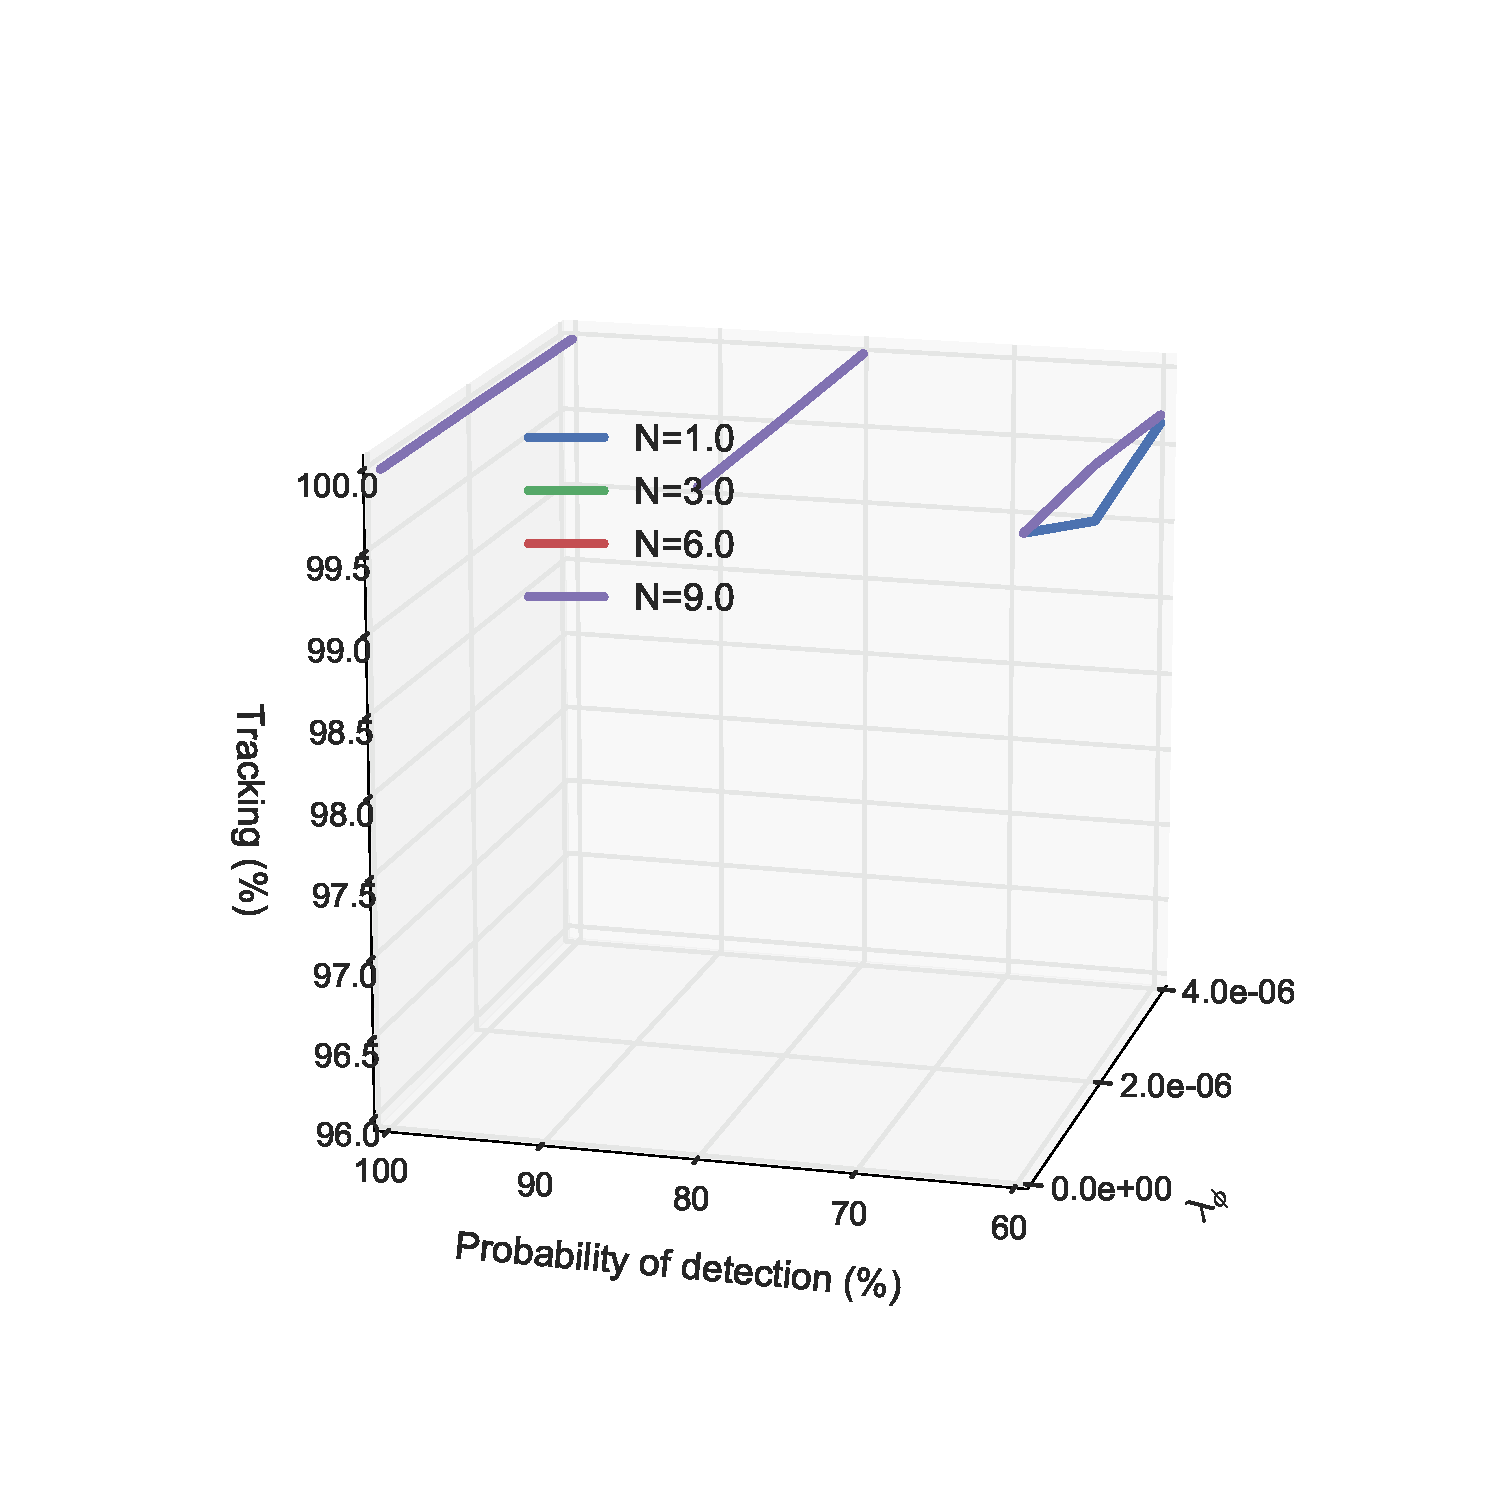
\includegraphics{Figures/plots/Scenario4_Tracking-TrackingPercentage.pdf}
\caption{Scenario 4 --- Tracking percentage}\label{fig:scenario4_tracking_percentage}
\end{figure}
\clearpage{}

\subsection{Effect of smoothing}
\Cref{fig:scenario0_tracking_correctness,fig:scenario1_tracking_correctness,fig:scenario2_tracking_correctness,fig:scenario3_tracking_correctness,fig:scenario4_tracking_correctness} show the \gls{rms} error between the true and estimated tracks for \(\lambda_\phi = 1\cdot10^{-5}\) with and without Kalman smoothing. From these we can see that the larger window sizes have higher errors, most likely since they are dead reckoning for a longer period and still able to converge back to the true track. We can also see that a larger window size gains more on smoothing and leads to better smoothed track overall,  giving the \gls{cas} more accurate tracks to work on.
\begin{figure}[H]
\centering
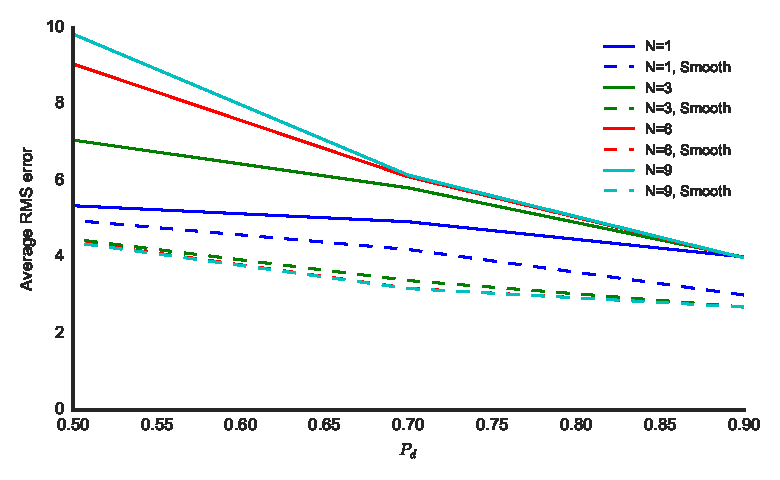
\includegraphics{Figures/plots/Scenario0_Tracking-TrackingCorrectness.pdf}
\caption{Scenario 0 --- Tracking Correctness}\label{fig:scenario0_tracking_correctness}
\end{figure}

\begin{figure}
\centering
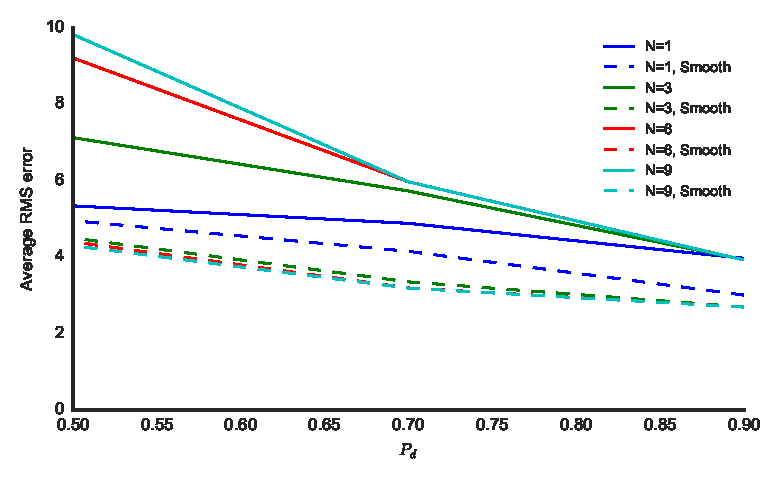
\includegraphics{Figures/plots/Scenario1_Tracking-TrackingCorrectness.pdf}
\caption{Scenario 1 --- Tracking Correctness}\label{fig:scenario1_tracking_correctness}
\end{figure}
\begin{figure}
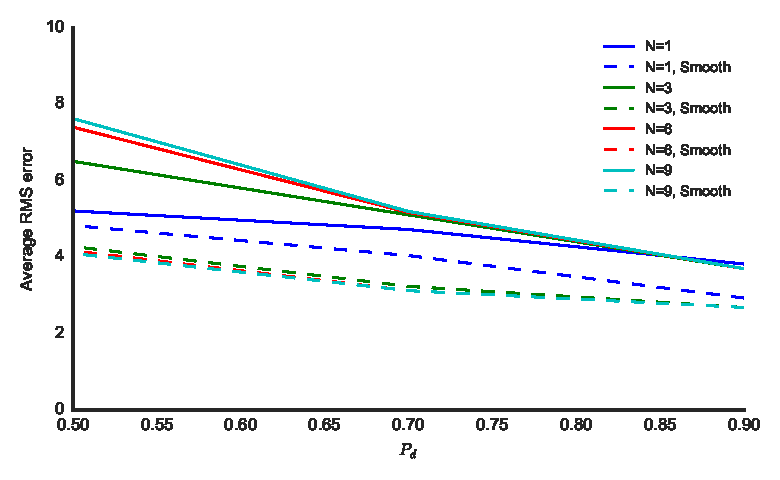
\includegraphics{Figures/plots/Scenario2_Tracking-TrackingCorrectness.pdf}
\caption{Scenario 2 --- Tracking Correctness}\label{fig:scenario2_tracking_correctness}
\end{figure}
\begin{figure}
\centering
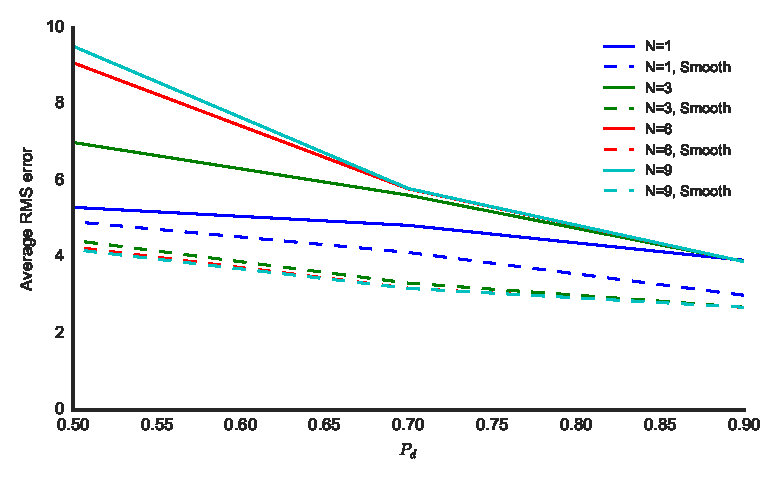
\includegraphics{Figures/plots/Scenario3_Tracking-TrackingCorrectness.pdf}
\caption{Scenario 3 --- Tracking Correctness}\label{fig:scenario3_tracking_correctness}
\end{figure}
\begin{figure}
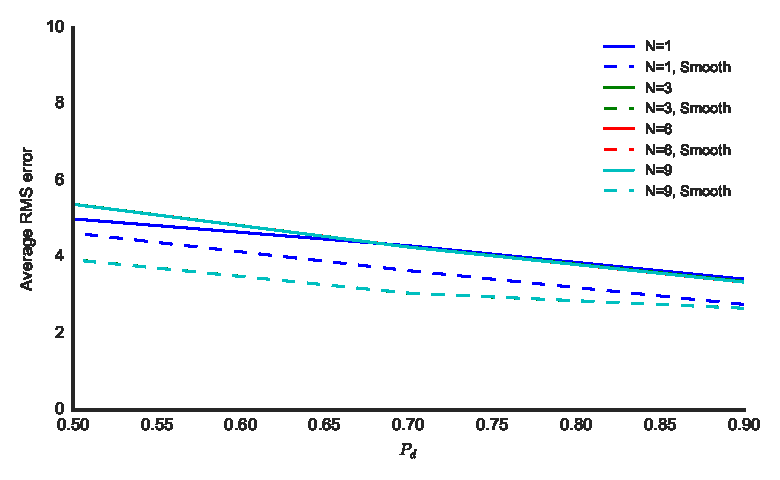
\includegraphics{Figures/plots/Scenario4_Tracking-TrackingCorrectness.pdf}
\caption{Scenario 4 --- Tracking Correctness}\label{fig:scenario4_tracking_correctness}
\end{figure}
\clearpage{}

\subsection{Runtime performance}
\Cref{fig:scenario0_tracking_runtime,fig:scenario1_tracking_runtime,fig:scenario2_tracking_runtime,fig:scenario3_tracking_runtime,fig:scenario4_tracking_runtime} show the average runtime for an iteration for scenario 0 --- 4. From these we can see the very expected increase in runtime as the window size increases, and that the \gls{ais} scenarios have a steeper increase that the pure radar scenario. This is caused by an increase in the number of nodes in the forest and a not as fast implementation of the AIS measurements processing as radar measurements, primarily caused by the large amount of steps in the AIS processing.

\begin{figure}[H]
\centering
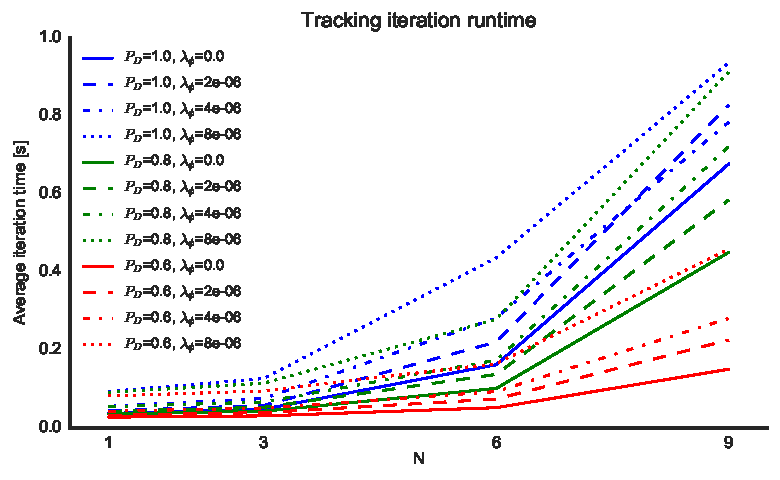
\includegraphics{Figures/plots/Scenario0_Tracking-Runtime.pdf}
\caption{Scenario 0 --- Tracking runtime}\label{fig:scenario0_tracking_runtime}
\end{figure}

\begin{figure}
\centering
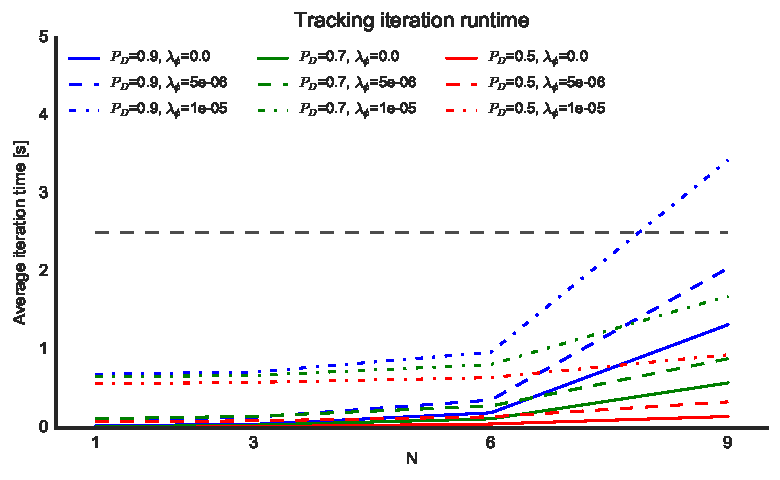
\includegraphics{Figures/plots/Scenario1_Tracking-Runtime.pdf}
\caption{Scenario 1 --- Tracking runtime}\label{fig:scenario1_tracking_runtime}

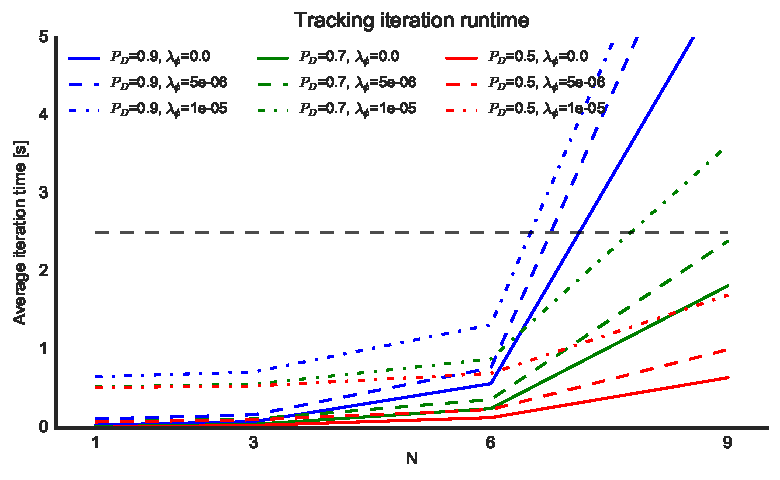
\includegraphics{Figures/plots/Scenario2_Tracking-Runtime.pdf}
\caption{Scenario 2 --- Tracking runtime}\label{fig:scenario2_tracking_runtime}
\end{figure}

\begin{figure}
\centering
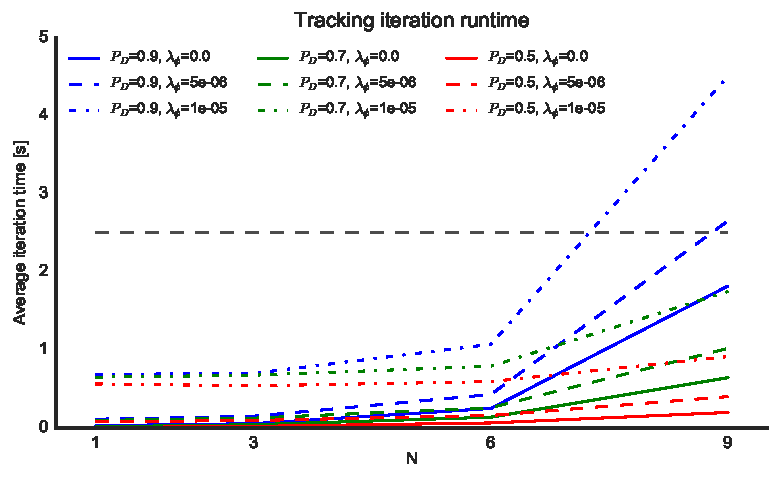
\includegraphics{Figures/plots/Scenario3_Tracking-Runtime.pdf}
\caption{Scenario 3 --- Tracking runtime}\label{fig:scenario3_tracking_runtime}

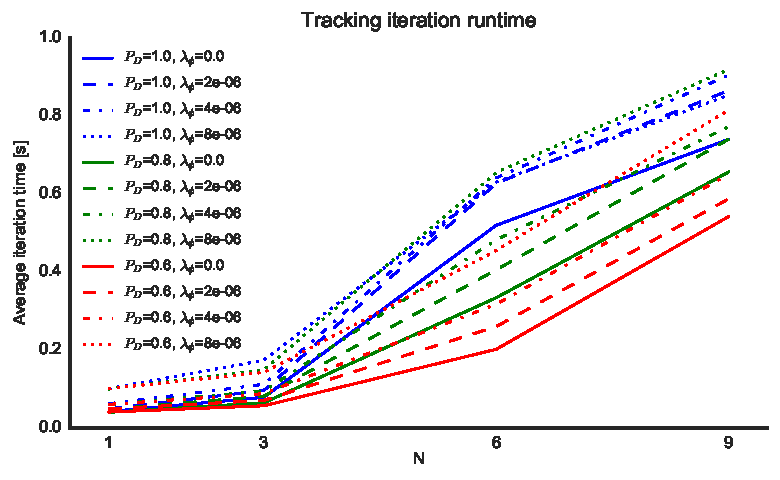
\includegraphics{Figures/plots/Scenario4_Tracking-Runtime.pdf}
\caption{Scenario 4 --- Tracking runtime}\label{fig:scenario4_tracking_runtime}
\end{figure}
